%%%%%%%%%%%%%%%%%%%%%%%%%%%%%%%%%%%%%%%%%%%%%%%%%%%%%%%%%%%%%
%% Begin exercise %%
%%%%%%%%%%%%%%%%%%%%%%%%%%%%%%%%%%%%%%%%%%%%%%%%%%%%%%%%%%%%%
\ex{Rectifiers}

%%%%%%%%%%%%%%%%%%%%%%%%%%%%%%%%%%%%%%%%%%%%%%%%%%%%%%%%%%%%%
%% Task 1: M3C converter at a RL-load                     %%
%%%%%%%%%%%%%%%%%%%%%%%%%%%%%%%%%%%%%%%%%%%%%%%%%%%%%%%%%%%%%

\task{M3C converter at an RL-load}
A controlled three-pulse midpoint circuit feeds an ohmic-inductive load. The load inductance $L$ is large, such that a pure direct current $I_\mathrm{2}$ is taken from the converter. The load resistance is $R = \SI{5}{\Omega}$. The converter transformer 
is connected to the symmetrical three-phase network with $U_\mathrm{N} = \SI{\nicefrac{230}{400}}{\volt} $ (effective value of phase voltage / line-to-line voltage). The secondary side phase voltages point an effective value of 
$U_\mathrm{1i} = \SI{230}{\volt}, \forall i=a,b,c$. The thyristors and commutation can be assumed to be ideal.

%%%%%%%%%%%%%%%%%%%%%%%%%%%%%%%%%%%%%%%%%%%%%%%%%%%%%%%%%%%%%%%%%%%%%%%
 % M3C rectifier with RL Load
%%%%%%%%%%%%%%%%%%%%%%%%%%%%%%%%%%%%%%%%%%%%%%%%%%%%%%%%%%%%%%%%%%%%%%%
\begin{figure}[htb]
  \begin{center}
    \begin{circuitikz}
      \def\vd{1cm} % vertical distance inductors
      \def\htraf{0.75cm} % horizontal distance transformer coils
      \draw (0,0) to [short, o-] ++(0.5,0) coordinate (L1astart) to [short] ++(0.5,0) to [L] ++(2,0) coordinate (L1aend)
      (0,-1*\vd) to [short, o-] ++(1,0) coordinate (L1bstart) to [L] ++(2,0) coordinate (L1bend)
      (0,-2*\vd) to [short, o-] ++(1,0) coordinate (L1cstart) to [L] ++(2,0) coordinate (L1cend) -- ++(0,-0.5*\vd) to (\tikztostart -| L1astart) 
      to [crossing] ++(0, 1*\vd) to [crossing] ++(0, 1*\vd) to [short, -*] (L1astart)
      (L1aend) -- ++(0,-0.5*\vd) to (\tikztostart -| L1bstart) to [short, -*] (L1bstart)
      (L1bend) -- ++(0,-0.5*\vd) to (\tikztostart -| L1cstart) to [short, -*] (L1cstart);
      \draw let \p1=(L1aend) in (\x1 + \htraf, \y1) coordinate (L2astart) to [L, v^<=$u_{1\mathrm{a}}(t)$, voltage = straight] ++(2,0) to [short, i=$i_{1\mathrm{a}}(t)$] ++(0.5,0) coordinate (L2aend);
      \draw let \p1=(L1bend) in (\x1 + \htraf, \y1) coordinate (L2bstart) to [L, v^<=$u_{1\mathrm{b}}(t)$, voltage = straight] ++(2,0) to [short, i=$i_{1\mathrm{b}}(t)$] ++(0.5,0) coordinate (L2bend);
      \draw let \p1=(L1cend) in (\x1 + \htraf, \y1) coordinate (L2cstart) to [L, v^<=$u_{1\mathrm{c}}(t)$, voltage = straight] ++(2,0) to [short, i=$i_{1\mathrm{c}}(t)$] ++(0.5,0)  coordinate (L2cend);
      \draw (L2astart) to [short, -*] (L2bstart) to [short, -*] (L2cstart) -- ++(0, -1*\vd) -- ++(5,0) coordinate (Rend);
      \draw[double, double distance=3pt, thick] let \p1=(L1aend), \p2=(L2cstart) in (\x1/2+\x2/2, \y1) -- (\x1/2+\x2/2, \y2);
      \draw (L2aend) to [thyristor] ++(1.25,0) coordinate (D1end);
      \draw (L2bend) to [thyristor] ++(1.25,0) coordinate (D2end);
      \draw (L2cend) to [thyristor] ++(1.25,0) coordinate (D3end) to [short, -*] (D2end) to [short, -*] (D1end);
      \draw (D1end) to [short] ++(0.5,0) coordinate (u2) to [short, i=$i_2(t)$] ++(0.75,0) to [L, l=$L$] ++(2,0) coordinate (Ctop) to [short, i = $i_\mathrm{R}(t)$] ++(1.5,0) to [R, l=$R$] (Rend -| \tikztostart) to (Rend); 
      \draw (u2) to [open, v^>=$\hspace{0.5cm}u_2(t)$, voltage = straight] (Rend -| \tikztostart);
    \end{circuitikz}%
  \end{center}
  \caption{M3C topology with an input three-phase transformer and an RL-load.}
  \label{fig:M3C_topology_RL_no_filter}
\end{figure}


% Subtask1
\subtask{Calculate the firing angle $\alpha$, so that an active power of $P = \SI{6}{\kilo\watt}$ is delivered to the load. How big is the load current $i_\mathrm{2} = I_\mathrm{2}$?}
% Subtask2
\subtask{Draw the normalized control characteristic curve $\nicefrac{U_\mathrm{2}(\alpha)}{U_\mathrm{2}(\alpha=0)}$ and plot the  operating point $P = \SI{6}{\kilo\watt}$ at $R = \SI{5}{\Omega}$.}
% Subtask3
\subtask{Draw the curve of the converters' output voltage $u_\mathrm{2}(t)$ for the calculated control angle $\alpha$ from subtask 6.1.1.}
\subtask{Calculate the effective value $I^\mathrm{(1)}_\mathrm{1a}$ of the fundamental current component $i^\mathrm{(1)}_\mathrm{1a}(t)$ and draw that fundamental component. How big is the phase shift $\varphi_\mathrm{1a}$ between $u_\mathrm{1a}(t)$ and $i^\mathrm{(1)}_\mathrm{1a}(t)$.}
\subtask{Calculate the fundamental reactive power $Q^\mathrm{(1)}_\mathrm{1}$.}

%%%%%%%%%%%%%%%%%%%%%%%%%%%%%%%%%%%%%%%%%%%%%%%%%%%%%%%%%%%%%
%% Task 2: B6C converter at a motor load                   %%
%%%%%%%%%%%%%%%%%%%%%%%%%%%%%%%%%%%%%%%%%%%%%%%%%%%%%%%%%%%%%
\task{B6C converter at a motor load}

In a lifting drive, a permanent magnet DC motor is supplied by a B6C converter circuit. The B6C-topology is connected to the three-phase network.
With the assumption of $L\rightarrow\infty$ the motor operates with constant nominal current and constant nominal voltage when lifting as well as lowering the load.
This corresponds to a terminal voltage of $u_\mathrm{mot,up}(t)=U_\mathrm{mot}$ when lifting the load and $u_\mathrm{mot,down}(t)=-U_\mathrm{mot}$ when lowering it.
In order to generate the necessary torque, the motor absorbs the current $i_\mathrm{mot}(t)=I_\mathrm{mot}$.

%%%%%%%%%%%%%%%%%%%%%%%%%%%%%%%%%%%%%%%%%%%%%%%%%%%%%%%%%%%%%%%%%%%%%%%
 % B2U rectifier with capacitive output filtering
%%%%%%%%%%%%%%%%%%%%%%%%%%%%%%%%%%%%%%%%%%%%%%%%%%%%%%%%%%%%%%%%%%%%%%%
    \begin{figure}[htb]
        \begin{center}
            \begin{circuitikz}
                \def\vd{1.5cm} % vertical distance AC sources
                \def\hd{1.5cm} % horizontal distance diode bridge
                \def\h1d{5.0cm} % horizontal position first diode string
                % Base point for voltage supplies
                \coordinate (orig) at (0,0);
                % Voltage sources and neutral connection
                \draw 
                % draw the neutral connection
                (0,0) to [short, -*] ++(0,-1.5) to [short] ++(0,-1.5)
                % draw first phase ua
                (0,0) to [sinusoidal voltage source, v^<=$u_{1\mathrm{a}}$] ++(1.5, 0) to [short, i=$i_{1\mathrm{a}}(t)$]++(0.75,0) -- ++(0.25,0) coordinate (A)
                % draw second phase ub
                (0,-1*\vd) to [sinusoidal voltage source, v^<=$u_{1\mathrm{b}}$] ++(1.5, 0) to [short, i=$i_{1\mathrm{b}}(t)$]++(0.75,0) -- ++(0.25,0) coordinate (B)
                % draw third phase uc
                (0,-2*\vd) to [sinusoidal voltage source, v^<=$u_{1\mathrm{c}}$] ++(1.5,0) to [short, i=$i_{1\mathrm{c}}(t)$]++(0.75,0) -- ++(0.25,0) coordinate (C)
                %thyristor bridge
                % Add thyristor T1
                (\h1d,0) to [thyristor, l=$T_1$, name=D1] ++(0,1.25) coordinate (D1top)
                % Add thyristor T2
                (\h1d,-4.25) coordinate (D2bot) to [thyristor, l=$T_2$, name=D2] ++(0,1.25) to [short] (\h1d, 0)
                % Add connection to junction A
                (\h1d, 0) to [short, *-] (A)
                % Add thyristor T3
                (\h1d+\hd,0) to [thyristor, l=$T_3$, name=D3] ++(0,1.25) coordinate (D3top)
                % Add thyristor T4
                (\h1d+\hd,-4.25) coordinate (D4bot) to [thyristor, l=$T_4$, name=D4] ++(0,1.25) to [short] (\h1d+\hd, 0)
                % Add thyristor T5
                (\h1d+2*\hd,0) to [thyristor, l=$T_5$, name=D5] ++(0,1.25) coordinate (D5top)
                % Add thyristor T6
                (\h1d+2*\hd,-4.25) coordinate (D6bot) to [thyristor, l=$T_6$, name=D6] ++(0,1.25) to [short] (\h1d+2*\hd, 0)
                % Add connection to junction B
                (B -| D3) to [crossing, *-, mirror] ++(-2*\hd,0) -- (B)
                % Add connection to junction C
                (C -| D5) to [short, *-] ++(-\hd/2,0) to [crossing, mirror] ++(-\hd,0) to [crossing, mirror] ++(-\hd,0) -- (C)
                % Add wire T1-T3-T5
                (D1top) to [short, -*] (D3top) to [short, -*] (D5top) to [short, -] ++(0.5,0) coordinate (jL1)
                % Add inductor L and motor current
                (jL1) to [L, l=$L$, name = L] ++(2,0) to [short,i=$\overline{i}_\mathrm{mot}$] ++(0.5,0)  coordinate (jL2)
                % Add DC-motor and motor voltage
                (jL2) to [R, l=$R$, name = R, v_>=$\overline{u}_\mathrm{mot}$, voltage = straight]  (D6bot -| \tikztostart) to (D6bot)
                % Add wire T2-T3-T6
                (D2bot) to [short, -*] (D4bot) to [short, -*] (D6bot)
                % Add voltage arrow u2(t) between Dtop and Dbot
                (jL1) to [open, v^>=$\hspace{0.5cm}u_2(t)$, voltage = straight] (D6bot-|jL1)                
                % Add voltage arrow u2+n(t) between Dtop and neutral
                (D1top) ++(-0.2,0) to [open, v_>=$u_\mathrm{2,p}(t)$, voltage = straight] ++(-5.5,0)
                % Add voltage arrow u2-n(t) between Dbot and neutral
                (D2bot) ++(-0.2,0) to [open, v_>=$u_\mathrm{2,m}(t)$, voltage = straight] ++(-5.5,0)
                % Add voltage arrow between AC source a and b
                (A) to [open, v^>=$\hspace{0.75cm}u_{1\mathrm{ab}}(t)$, voltage = straight] (B)
                % Add voltage arrow between AC source b and c
                (B) to [open, v^>=$\hspace{0.75cm}u_{1\mathrm{bc}}(t)$, voltage = straight] (C)
                % Add voltage arrow between AC source a and c
                (-0.5,-2*\vd) to [open, v^>=$u_{1\mathrm{ca}}(t)\hspace{0.75cm}$, voltage = straight] (-0.5,0);
            \end{circuitikz}
        \end{center}
        \caption{B6C converter at a motor load}
        \label{fig:B6C_topology_WithMotor}
    \end{figure}




\begin{table}[ht]
    \centering  % Zentriert die Tabelle
    \begin{tabular}{ll}
        \toprule
        Input voltages: & three-phase system with $\hat{u}_\mathrm{1} = $ \\ %\square{2}\SI{230}{\volt}$  \\
        Nom. motor current: & $I_{\mathrm{mot}} = \SI{20}{\ampere}$ \\
        Nom. motor voltage: & $U_\mathrm{mot} = \SI{466}{\volt}$ \\ 
        Frequency: & $f= \SI{50}{\hertz}$ \\ 
        \bottomrule
    \end{tabular}
    \caption{Parameters of the lifting drive with B6C converter.}  
    \label{table:ex06_Task2_ParametersOfTheCircuit}
\end{table}


% Subtask1
\subtask{Calculate the firing angle $\alpha_\mathrm{up}$ required for raising and the firing angle $\alpha_\mathrm{down}$ for lowering the load 
to operate the motor at rated voltage. The average voltage $\overline{u}_\mathrm{2}$  as a function of the firing angle $\alpha$ shall be determined 
by integrating the instantaneous output voltage $u_\mathrm{2}(t)$.}
% Subtask2
\subtask{Sketch following waveformes fpr tje two calculated firing angles $\alpha_\mathrm{up}$ and $\alpha_\mathrm{down}$:
\begin{itemize}
    \item The output voltage $u_\mathrm{2,p}(t)$ and $u_\mathrm{2,m}(t)$ of the two partial converters (reference point is neutral)
          and shade the effective voltage-time area for the two cases (raising and lowing load).
    \item The output voltage $u_\mathrm{2}(t)$ and the mean voltage $\overline{u}_\mathrm{2}(t)$.
    \item The current $i_\mathrm{1a}(t)$ and it's fundamental amplitude.
    \item The voltage of thyristor $u_\mathrm{T1}(t)$.
    \item Mark the conduction intervals of $T_\mathrm{1}$...$T_\mathrm{6}$.
\end{itemize}  
}
\begin{solutionblock}
%%%%%%%%%%%%%%%%%%%%%%%%%%%%%%%%%%%%%%%%%%%%%%%%%%%%%%%%%%%%%%%%%%%%%%%%%%
% Signals of u2,p u2,m for raising load
%%%%%%%%%%%%%%%%%%%%%%%%%%%%%%%%%%%%%%%%%%%%%%%%%%%%%%%%%%%%%%%%%%%%%%%%%%
\begin{solutionfigure}[htb]

 %   \documentclass{standalone}
 %   \usepackage{pgfplots}
 %   \pgfplotsset{compat=1.18} % Kompatibilität für neuere Versionen
        \centering
        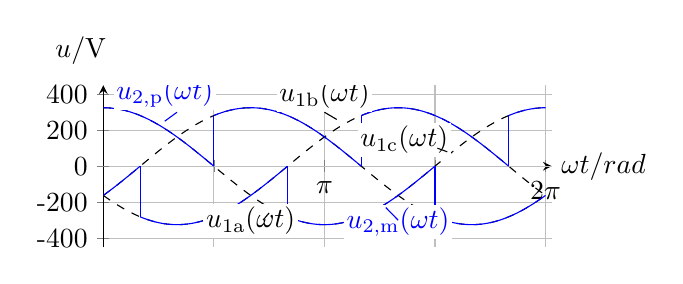
\begin{tikzpicture}
            \begin{axis}[
                % x/y range adjustment
                xmin=0, xmax=365,
                ymin=-450, ymax=450,
                samples=500,
                axis y line=center,
                axis x line=middle,
                extra y ticks=0,
                % Label text
                xlabel={$\omega t / \text{rad}$},,
                ylabel={$u/\mathrm{V}$},
                % Label adjustment
                x label style={at={(axis description cs:1,0.5)},anchor=west},
                y label style={at={(axis description cs:-.05,.97)},anchor=south,yshift=0.2cm},
                width=0.6\textwidth,
                height=0.3\textwidth,
                % x-Ticks
                xtick={0,90,180,270,360},
                xticklabels={,,$\pi$,,$2\pi$},
                xticklabel style = {anchor=north},
                % y-Ticks
                ytick={400,200,0,-200,-400},
                yticklabels={400,200,0,-200,-400},
                yticklabel style = {anchor=east},
                % Grid layout
                grid,
                %grid style={line width=.1pt, draw=gray!10},
                %major grid style={line width=.2pt,draw=gray!90},
            ]
            % Voltage u1a(wt), u1b(wt) u1c(wt)
            \addplot[black, domain= 0:360,dashed] {325*cos(x)};                
            \addplot[black, domain= 0:360,dashed] {325*cos(x+120)};                
            \addplot[black, domain= 0:360,dashed] {325*cos(x+240)}; 
            % Voltage u2p(wt)
            \addplot[blue, domain= 0:90] {325*cos(x)};                
            \addplot[blue, domain= 90:210] {325*cos(x+240)};                
            \addplot[blue, domain= 210:330] {325*cos(x+120)};
            \addplot[blue, domain= 330:360] {325*cos(x)};                
            \addplot[color=blue,solid] coordinates{
                (90,0)
                (90, 281.4)
            };     
            \addplot[color=blue,solid] coordinates{
                (210,0)
                (210, 281.4)
            };     
            \addplot[color=blue,solid] coordinates{
                (330,0)
                (330, 281.4)
            };     
         
            % Voltage u2m(wt)
            \addplot[blue, domain= 0:30] {325*cos(x+240)};                
            \addplot[blue, domain= 30:150] {325*cos(x+120)};                
            \addplot[blue, domain= 150:270] {325*cos(x)};                
            \addplot[blue, domain= 270:360] {325*cos(x+240)};
            \addplot[color=blue,solid] coordinates{
                (30,0)
                (30, -281.4)
            };     
            \addplot[color=blue,solid] coordinates{
                (150,0)
                (150, -281.4)
            };     
            \addplot[color=blue,solid] coordinates{
                (270,0)
                (270, -281.4)
            };     
        
            % Label of u1c
            \node[black, fill=white, inner sep = 1pt, anchor = south] at (axis cs:245,50) {$u_{\mathrm{1c}}(\omega t)$};
            % Line to u1a
            \draw[thin, black] (272,100) -- (280,80); 
            % Label of u1a
            \node[black, fill=white, inner sep = 1pt, anchor = south] at (axis cs:120,-400) {$u_{\mathrm{1a}}(\omega t)$};
            % Line to u1a
            \draw[thin, black] (130,-300) -- (135,-260);            
            % Label of u1b
            \node[black, fill=white, inner sep = 1pt, anchor = south] at (axis cs:180,300) {$u_{\mathrm{1b}}(\omega t)$};
            % Line to u1b
            \draw[thin, black] (180,300) -- (190,260);
            % Label of u2,p
            \node[blue, fill=white, inner sep = 1pt, anchor = south] at (axis cs:50,310) {$u_{\mathrm{2,p}}(\omega t)$};
            % Line to u2,p
            \draw[thin, blue] (60,300) -- (50,250);
            % Label of u2,m
            \node[blue, fill=white, inner sep = 1pt, anchor = south] at (axis cs:240,-410) {$u_{\mathrm{2,m}}(\omega t)$};
            % Line to u2,m
            \draw[thin, blue] (240,-300) -- (230,-230);
        \end{axis}     
        \end{tikzpicture}
        \caption{Output voltage $u_\mathrm{2,p}(t)$ and $u_\mathrm{2,m}(t)$ for raising load.}
        \label{sfig:ex06_Voltage_u2pmn_Raise}
\end{solutionfigure}

%%%%%%%%%%%%%%%%%%%%%%%%%%%%%%%%%%%%%%%%%%%%%%%%%%%%%%%%%%%%%%%%%%%%%%%%%%
% Signals of u2,p u2,m for lowing load
%%%%%%%%%%%%%%%%%%%%%%%%%%%%%%%%%%%%%%%%%%%%%%%%%%%%%%%%%%%%%%%%%%%%%%%%%%
\begin{solutionfigure}[htb]

 %   \documentclass{standalone}
 %   \usepackage{pgfplots}
 %   \pgfplotsset{compat=1.18} % Kompatibilität für neuere Versionen
        \centering
        \begin{tikzpicture}
            \begin{axis}[
                % x/y range adjustment
                xmin=0, xmax=368,
                ymin=-500, ymax=500,
                samples=500,
                axis y line=center,
                axis x line=middle,
                extra y ticks=0,
                % Label text
                xlabel={$\omega t / \text{rad}$},,
                ylabel={$u/\mathrm{V}$},
                % Label adjustment
                x label style={at={(axis description cs:1,0.5)},anchor=west},
                y label style={at={(axis description cs:-.05,.97)},anchor=south,yshift=0.2cm},
                width=0.6\textwidth,
                height=0.3\textwidth,
                % x-Ticks
                xtick={0,90,180,270,360},
                xticklabels={,,$\pi$,,$2\pi$},
                xticklabel style = {anchor=north},
                % y-Ticks
                ytick={400,200,0,-200,-400},
                yticklabels={400,200,0,-200,-400},
                yticklabel style = {anchor=east},
                % Grid layout
                grid,
                thick,
                %grid style={line width=.1pt, draw=gray!10},
                %major grid style={line width=.2pt,draw=gray!90},
            ]
            % Voltage u1a(wt), u1b(wt) u1c(wt)
            \addplot[black, domain= 0:360,dashed,name path = u1a] {325*cos(x)};                
            \addplot[black, domain= 0:360,dashed,name path = u1b] {325*cos(x-120)};                
            \addplot[black, domain= 0:360,dashed,name path = u1c] {325*cos(x-240)}; 
            % Voltage u2p(wt)
            \addplot[signalalpha, domain= 0:30] {325*cos(x)};                
            \addplot[signalalpha, domain= 30:150] {325*cos(x-120)};
            \addplot[signalalpha, domain= 150:270] {325*cos(x-240)};                
            \addplot[signalalpha, domain= 270:360] {325*cos(x)};                
            \addplot[color=signalalpha,solid] coordinates{
                (30,0)
                (30, 281.4)
            };     
            \addplot[color=signalalpha,solid] coordinates{
                (150,0)
                (150, 281.4)
            };     
            \addplot[color=signalalpha,solid] coordinates{
                (270,0)
                (270, 281.4)
            };     
    
           % Average u1p 
           \addplot[signalalpha,domain= 0:360,dashed, name path = u2pavg] {-233}; 
            
            % Voltage u2m(wt)
            \addplot[signalalpha, domain= 0:90] {325*cos(x+120)};                
            \addplot[signalalpha, domain= 90:210] {325*cos(x)};                
            \addplot[signalalpha, domain= 210:330] {325*cos(x+240)};
            \addplot[signalalpha, domain= 330:360] {325*cos(x+120)};
            \addplot[color=signalalpha,solid] coordinates{
                (90,0)
                (90, -281.4)
            };     
            \addplot[color=signalalpha,solid] coordinates{
                (210,0)
                (210, -281.4)
            };     
            \addplot[color=signalalpha,solid] coordinates{
                (330,0)
                (330, -281.4)
            };             
 
            % Average u1m 
            \addplot[signalalpha,domain= 0:360,dashed, name path = u2mavg] {233}; 

            % Shade areas of T1,T3,T5
            \addplot[shadecolor, opacity=0.3] fill between[of=u1c and u2pavg, soft clip={domain=0:90}];
            \addplot[shadecolor, opacity=0.3] fill between[of=u1a and u2pavg, soft clip={domain=90:210}];
            \addplot[shadecolor, opacity=0.3] fill between[of=u1b and u2pavg, soft clip={domain=210:330}];
            \addplot[shadecolor, opacity=0.3] fill between[of=u1c and u2pavg, soft clip={domain=330:360}];

            % Shade areas of T2,T4,T5
            \addplot[shadecolor, opacity=0.3] fill between[of=u1a and u2mavg, soft clip={domain=0:30}];
            \addplot[shadecolor, opacity=0.3] fill between[of=u1b and u2mavg, soft clip={domain=30:150}];
            \addplot[shadecolor, opacity=0.3] fill between[of=u1c and u2mavg, soft clip={domain=150:270}];
            \addplot[shadecolor, opacity=0.3] fill between[of=u1a and u2mavg, soft clip={domain=270:360}];            
         
            % Label of u1a
            \node[black, fill=white, inner sep = 1pt, anchor = south] at (axis cs:120,50) {$u_{\mathrm{1a}}(\omega t)$};
            % Line to u1a
            \draw[ black] (90,100) -- (80,80);            
            % Label of u1b
            \node[black, fill=white, inner sep = 1pt, anchor = south] at (axis cs:240,50) {$u_{\mathrm{1b}}(\omega t)$};
            % Line to u1b
            \draw[ black] (210,100) -- (200,80);
            % Label of u1c
            \node[black, fill=white, inner sep = 1pt, anchor = south] at (axis cs:295,-175) {$u_{\mathrm{1c}}(\omega t)$};
            % Line to u1c
            \draw[ black] (265,-120) -- (258,-115);              
            % Label of u2,m
            \node[signalalpha, fill=white, inner sep = 1pt, anchor = south] at (axis cs:50,310) {$u_{\mathrm{2,m}}(\omega t)$};
            % Line to u2,m
            \draw[signalalpha] (60,300) -- (70,250);
            % Label of u2,p
            \node[signalalpha, fill=white, inner sep = 1pt, anchor = south] at (axis cs:240,-410) {$u_{\mathrm{2,p}}(\omega t)$};
            % Line to u2,p
            \draw[signalalpha] (240,-300) -- (250,-230);

            % Thyristor phases u2p
            % Label of T1
            \draw[<->,black, solid] (axis cs:90,-440) -- (axis cs:210,-440);
            \node[black, fill=white, inner sep = 1pt, anchor = south] at (axis cs:170,-500) {$\mathrm{T_1}$};
            % Label of T3
            \draw[<->,black, solid] (axis cs:210,-440) -- (axis cs:330,-440);
            \node[black, fill=white, inner sep = 1pt, anchor = south] at (axis cs:300,-500) {$\mathrm{T_3}$};
            % Label of T5
            \draw[<-,black, solid] (axis cs:330,-440) -- (axis cs:360,-440);
            \draw[->,black, solid] (axis cs:0,-440) -- (axis cs:90,-440);
            \node[black, fill=white, inner sep = 1pt, anchor = south] at (axis cs:30,-500) {$\mathrm{T_5}$};


            % Thyristor phases u2m
            % Label of T4
            \draw[<->,black, solid] (axis cs:30,460) -- (axis cs:150,460);
            \node[black, fill=white, inner sep = 1pt, anchor = south] at (axis cs:100,400) {$\mathrm{T_4}$};
            % Label of T6
            \draw[<->,black, solid] (axis cs:150,460) -- (axis cs:270,460);
            \node[black, fill=white, inner sep = 1pt, anchor = south] at (axis cs:200,400) {$\mathrm{T_6}$};
            % Label of T2
            \draw[<-,black, solid] (axis cs:270,460) -- (axis cs:360,460);
            \draw[->,black, solid] (axis cs:0,460) -- (axis cs:30,460);
            \node[black, fill=white, inner sep = 1pt, anchor = south] at (axis cs:330,400) {$\mathrm{T_2}$};

        \end{axis}     
        \end{tikzpicture}
        \caption{Output voltage $u_\mathrm{2,p}(t)$ and $u_\mathrm{2,m}(t)$ for lowering the load.}
        \label{sfig:ex06_Voltage_u2pm_Down}
\end{solutionfigure}

%%%%%%%%%%%%%%%%%%%%%%%%%%%%%%%%%%%%%%%%%%%%%%%%%%%%%%%%%%%%%%%%%%%%%%%%%%
% Signal of u2 for raising and lowing load
%%%%%%%%%%%%%%%%%%%%%%%%%%%%%%%%%%%%%%%%%%%%%%%%%%%%%%%%%%%%%%%%%%%%%%%%%%
\begin{solutionfigure}[htb]

 %   \documentclass{standalone}
 %   \usepackage{pgfplots}
 %   \pgfplotsset{compat=1.18} % Kompatibilität für neuere Versionen
        \centering
        \begin{tikzpicture}
            \begin{axis}[
                % x/y range adjustment
                xmin=0, xmax=368,
                ymin=-650, ymax=650,
                samples=500,
                axis y line=center,
                axis x line=middle,
                extra y ticks=0,
                % Label text
                xlabel={$\omega t / \text{rad}$},,
                ylabel={$u/\mathrm{V}$},
                % Label adjustment
                x label style={at={(axis description cs:1,0.5)},anchor=west},
                y label style={at={(axis description cs:-.05,.97)},anchor=south,yshift=0.2cm},
                width=0.6\textwidth,
                height=0.3\textwidth,
                % x-Ticks
                xtick={0,90,180,270,360},
                xticklabels={,,$\pi$,,$2\pi$},
                xticklabel style = {anchor=north},
                % y-Ticks
                ytick={600,400,200,0,-200,-400,-600},
                yticklabels={600,400,200,0,-200,-400,-600},
                yticklabel style = {anchor=east},
                % Grid layout
                grid,
                thick
                %grid style={line width=.1pt, draw=gray!10},
                %major grid style={line width=.2pt,draw=gray!90},
            ]
            % Voltage u1ab(wt), u1bc(wt) u1ca(wt)
            \addplot[black, domain= 0:360,dashed] {563*cos(x-30)};                
            \addplot[black, domain= 0:360,dashed] {563*cos(x+90)};                
            \addplot[black, domain= 0:360,dashed] {563*cos(x+210)}; 
            % Voltage -u1ab(wt), -u1bc(wt) -u1ca(wt)
            \addplot[black, domain= 0:360,dashed] {-563*cos(x-30)};                
            \addplot[black, domain= 0:360,dashed] {-563*cos(x+90)};                
            \addplot[black, domain= 0:360,dashed] {-563*cos(x+210)}; 
            % Voltage u2(wt) up
            \addplot[signalalpha, domain= 0:30] {-563*cos(x+210)};            
            \addplot[signalalpha, domain= 30:90] {563*cos(x-30)};                
            \addplot[signalalpha, domain= 270:330] {563*cos(x+90)};                
            \addplot[signalalpha, domain= 150:210] {563*cos(x+210)}; 
            \addplot[signalalpha, domain= 210:270] {-563*cos(x-30)};                
            \addplot[signalalpha, domain= 90:150] {-563*cos(x+90)};                
            \addplot[signalalpha, domain= 330:360] {-563*cos(x+210)};            
            \addplot[color=signalalpha,solid] coordinates{
                (30, 563)
                (30, 282)
            };     
            \addplot[color=signalalpha,solid] coordinates{
                (90, 563)
                (90, 282)
            };     
            \addplot[color=signalalpha,solid] coordinates{
                (150, 563)
                (150, 282)
            };     
            \addplot[color=signalalpha,solid] coordinates{
                (210, 563)
                (210, 282)
            };     
            \addplot[color=signalalpha,solid] coordinates{
                (270, 563)
                (270, 282)
            };     
            \addplot[color=signalalpha,solid] coordinates{
                (330, 563)
                (330, 282)
            };     
    
            % Voltage u2(wt) down
            \addplot[signalalpha, domain= 0:30] {-563*cos(x-30)};                
            \addplot[signalalpha, domain= 150:210] {563*cos(x-30)};                
            \addplot[signalalpha, domain= 30:90] {563*cos(x+90)};                
            \addplot[signalalpha, domain= 270:330] {563*cos(x+210)};            
            \addplot[signalalpha, domain= 330:360] {-563*cos(x-30)};                
            \addplot[signalalpha, domain= 210:270] {-563*cos(x+90)};                
            \addplot[signalalpha, domain= 90:150] {-563*cos(x+210)}; 
            \addplot[color=signalalpha,solid] coordinates{
                (30,-563)
                (30,-282)
            };     
            \addplot[color=signalalpha,solid] coordinates{
                (90,-563)
                (90,-282)
            };     
            \addplot[color=signalalpha,solid] coordinates{
                (150,-563)
                (150,-282)
            };     
            \addplot[color=signalalpha,solid] coordinates{
                (210,-563)
                (210,-282)
            };     
            \addplot[color=signalalpha,solid] coordinates{
                (270,-563)
                (270,-282)
            };     
            \addplot[color=signalalpha,solid] coordinates{
                (330,-563)
                (330,-282)
            };     
         
            % Label of +-u1ab
            \node[black, fill=white, inner sep = 1pt, anchor = south] at (axis cs:30,10) {$\pm u_{\mathrm{1ab}}$};
            % Line to +u1ab
            \draw[black] (30,140) -- (35,190);            
            % Line to -u1ab
            \draw[black] (30,-10) -- (35,-100);            
            % Label of +-u1bc
            \node[black, fill=white, inner sep = 1pt, anchor = south] at (axis cs:150,10) {$\pm u_{\mathrm{1bc}}$};
            % Line to +u1bc
            \draw[black] (150,140) -- (155,190);            
            % Line to -u1bc
            \draw[black] (150,-10) -- (155,-100);   
            % Label of +-u1ca
            \node[black, fill=white, inner sep = 1pt, anchor = south] at (axis cs:270,10) {$\pm u_{\mathrm{1ca}}$};
            % Line to +u1ca
            \draw[black] (270,140) -- (275,190);            
            % Line to -u1ca
            \draw[black] (270,-10) -- (275,-100);               
            % Label of u2up
            \node[signalalpha, fill=white, inner sep = 1pt, anchor = south] at (axis cs:120,210) {$u_{\mathrm{2 up}}$};
            % Line to u2,up
            \draw[signalalpha] (120,370) -- (125,440);
            % Label of u2down
            \node[signalalpha, fill=white, inner sep = 1pt, anchor = south] at (axis cs:240,-380) {$u_{\mathrm{2 dn}}$};
            % Line to u2,down
            \draw[signalalpha] (240,-380) -- (235,-430);
        \end{axis}     
        \end{tikzpicture}
        \caption{Output voltage $u_\mathrm{2 up}(\omega t)$ for raising and $u_\mathrm{2 dn}(\omega t)$ lowering the load.}
        \label{sfig:ex06_Voltage_u2up_down}
\end{solutionfigure}


\end{solutionblock}

% Subtask3
\subtask{Calculate the mean value $P$ of the instantaneous active power $p(t)$, the fundamental reactive power $q_\mathrm{1a}(t)$
and the fundamental apparent power $s_\mathrm{1a}(t)$. Represent $p_\mathrm{1a}$, $q_\mathrm{1a}$ and $s_\mathrm{1a}$ in the complex plane.
}
% Subtask4
\subtask{Calculate the $s_\mathrm{1a}$, $p_\mathrm{1a}$ and $q_\mathrm{1a}$ and the fundamental component $g_\mathrm{1a}=\frac{i_\mathrm{1a,eff}}{i_\mathrm{1a}}$
         and the power factor $\lambda$ as a function of the effective values $u_\mathrm{1a}$, $i_\mathrm{1a}$, $i_\mathrm{1a,eff}$ and $\alpha$.}
         